%%%%%%%%%%%%%%%%%%%%%%%%%%%%%%%%%%%%%%%%%
% Beamer Presentation
% LaTeX Template
% Version 1.0 (10/11/12)
%
% This template has been downloaded from:
% http://www.LaTeXTemplates.com
%
% License:
% CC BY-NC-SA 3.0 (http://creativecommons.org/licenses/by-nc-sa/3.0/)
%
%%%%%%%%%%%%%%%%%%%%%%%%%%%%%%%%%%%%%%%%%

%----------------------------------------------------------------------------------------
%	PACKAGES AND THEMES
%----------------------------------------------------------------------------------------

%\documentclass{beamer}
\documentclass[12pt, aspectratio=169]{beamer}
\usepackage{keynote-gradient-dark}

\mode<presentation> {

% The Beamer class comes with a number of default slide themes
% which change the colors and layouts of slides. Below this is a list
% of all the themes, uncomment each in turn to see what they look like.

%\usetheme{default}
%\usetheme{AnnArbor}
%\usetheme{Antibes}
%\usetheme{Bergen}
%\usetheme{Berkeley}
%\usetheme{Berlin}
%\usetheme{Boadilla}
%\usetheme{CambridgeUS}
%\usetheme{Copenhagen}
%\usetheme{Darmstadt}
%\usetheme{Dresden}
%\usetheme{Frankfurt}
%\usetheme{Goettingen}
%\usetheme{Hannover}
%\usetheme{Ilmenau}
%\usetheme{JuanLesPins}
%\usetheme{Luebeck}
%\usetheme{Madrid}
%\usetheme{Malmoe}
%\usetheme{Marburg}
%\usetheme{Montpellier}
%\usetheme{PaloAlto}
%\usetheme{Pittsburgh}
%\usetheme{Rochester}
%\usetheme{Singapore}
%\usetheme{Szeged}
%\usetheme{Warsaw}

% As well as themes, the Beamer class has a number of color themes
% for any slide theme. Uncomment each of these in turn to see how it
% changes the colors of your current slide theme.

%\usecolortheme{albatross}
%\usecolortheme{beaver}
%\usecolortheme{beetle}
%\usecolortheme{crane}
%\usecolortheme{dolphin}
%\usecolortheme{dove}
%\usecolortheme{fly}
%\usecolortheme{lily}
%\usecolortheme{orchid}
%\usecolortheme{rose}
%\usecolortheme{seagull}
%\usecolortheme{seahorse}
%\usecolortheme{whale}
%\usecolortheme{wolverine}

%\setbeamertemplate{footline} % To remove the footer line in all slides uncomment this line
%\setbeamertemplate{footline}[page number] % To replace the footer line in all slides with a simple slide count uncomment this line

%\setbeamertemplate{navigation symbols}{} % To remove the navigation symbols from the bottom of all slides uncomment this line
}

\usepackage{graphicx} % Allows including images
\usepackage{booktabs} % Allows the use of \toprule, \midrule and \bottomrule in tables

%--------------------------------------------------------------------------------
%	TITLE PAGE
%--------------------------------------------------------------------------------

\title[Memristive brain]{Memristive brain} % The short title appears at the bottom of every slide, the full title is only on the title page

\author[Max Talanov]{
  % 
\includegraphics[height=2cm]{ITIS_logo_bright}\\
  Max Talanov
} 
\institute[Neurolab, ITIS: KFU]% Your institution as it will appear on the bottom of every slide, may be shorthand to save space
{
ITIS/Neurobiology laboratory, KFU \\ % Your institution for the title page
\medskip
\textit{max.talanov@gmail.com} % Your email address
}
\date{\today} % Date, can be changed to a custom date

\begin{document}

\begin{frame}
\titlepage % Print the title page as the first slide
\end{frame}
%-------------------------------------------------------------------------------
% NeuCogAr
%-------------------------------------------------------------------------------

%------------------------------------------------
\section{NeuCogAr}
%------------------------------------------------
\begin{frame}
  \frametitle{NeuCogAr}
  \begin{figure}
    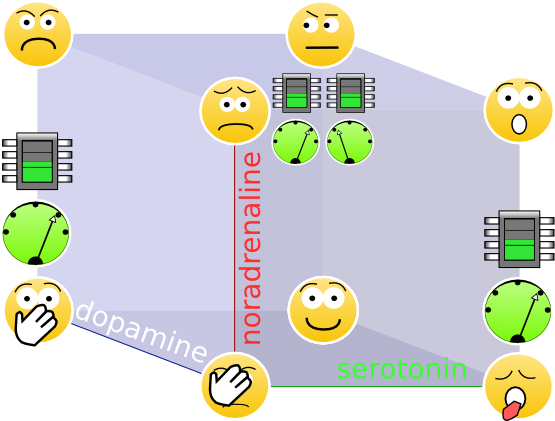
\includegraphics[width=0.55\linewidth]{cube_of_emotional_parameters_machine}
  \end{figure}
\end{frame}
%------------------------------------------------
\begin{frame}
  \frametitle{NeuCogAr: fear}
  \begin{figure}
    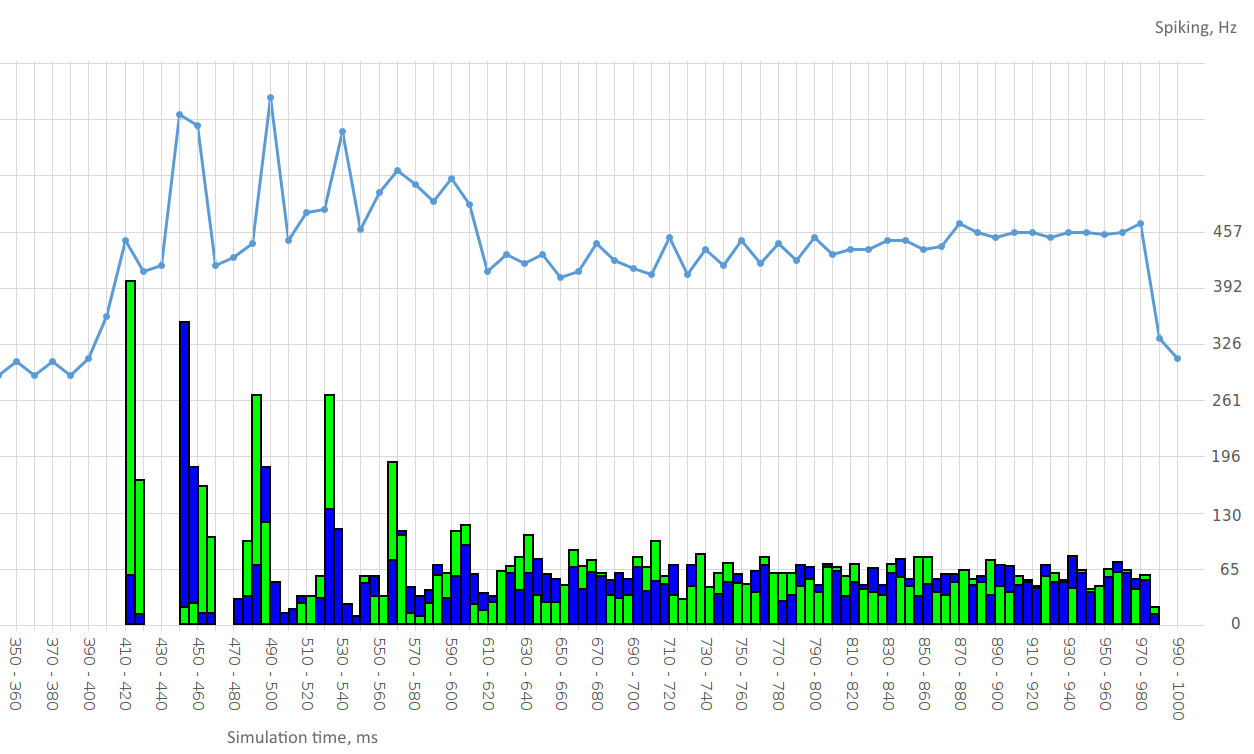
\includegraphics[width=0.8\linewidth]{resultBIG_short}
  \end{figure}
\end{frame}
%------------------------------------------------
\begin{frame}
  \frametitle{NeuCogAr: disgust}
  \begin{figure}
    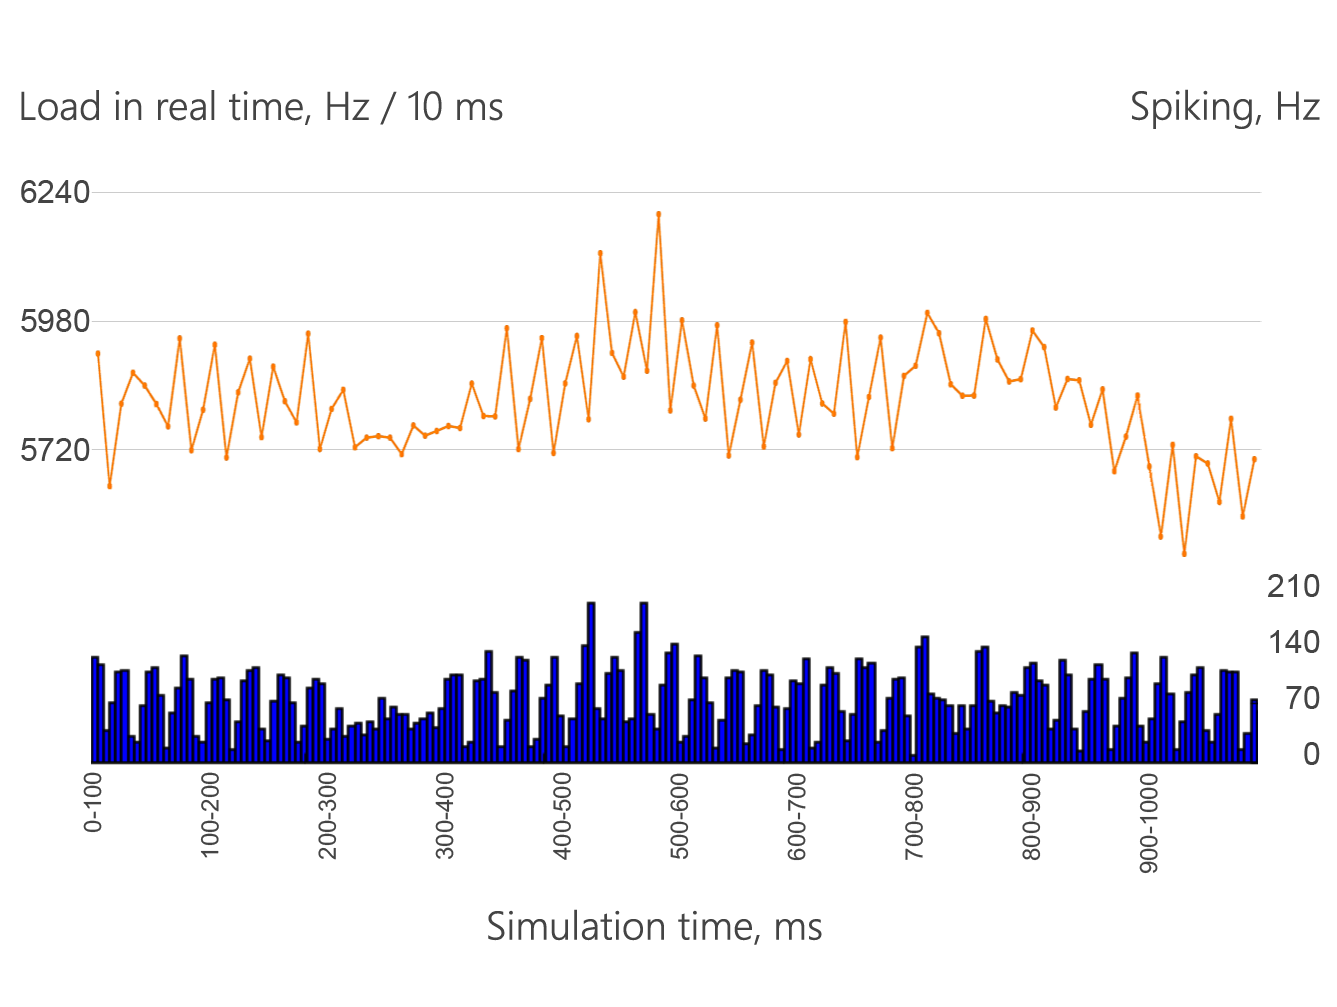
\includegraphics[width=0.7\linewidth]{5ht_results}
  \end{figure}
\end{frame}

%-------------------------------------------------------------------------------
%	Modulatory inhibitory memristive neuron schematic PRESENTATION SLIDES
%-------------------------------------------------------------------------------
\section{Robot dream}
%------------------------------------------------
\begin{frame}
  \frametitle{Robot dream: problem}
\begin{columns}[c]
\column{.5\textwidth} % Left column and width
\begin{itemize}
\item \emph{AR-601}: Intel Core i7; 8 GB
\item \emph{Nao}: Intel Atom @ 1.6 GHz
\item \emph{iCub}: Intel® Core™2 Duo; 2 GB
\end{itemize}

\emph{RIKEN} 2013: 1\% of human brain - 250 K-supercomputers (2.0 GHz 8-core SPARC64; 16 GB), slower than human brain in 1000 times.\\
\emph{Human brain project}: human brain -- 10 exaflop.

\column{.5\textwidth} % Right column and width
\begin{figure}
\includegraphics[width=1.0\linewidth]{RIKEN_AICS}
\end{figure}
\end{columns}
\end{frame}
%------------------------------------------------
\begin{frame}
  \frametitle{Robot dream: architecture}
  \begin{figure}
    
\includegraphics[width=0.99\linewidth]{reverse_translation}
  \end{figure}
\end{frame}


%-------------------------------------------------------------------------------
%	Modulatory inhibitory memristive neuron schematic PRESENTATION SLIDES
%-------------------------------------------------------------------------------


%------------------------------------------------
\section{Memristive brain}

%------------------------------------------------

\begin{frame}
  \frametitle{Memristive brain idea}
  \begin{figure}
    \includegraphics[width=0.4\linewidth]{mousebrainpink}
  \end{figure}
\end{frame}

%------------------------------------------------

\begin{frame}
  \frametitle{Modulatory, inhibitory memristive neuron}
  \begin{figure}
    \includegraphics[width=0.55\linewidth]{HL_mod_inh_mem_neuron}
  \end{figure}
\end{frame}

%------------------------------------------------

\begin{frame}
\frametitle{DA modulation: wiring schematic}
\begin{figure}
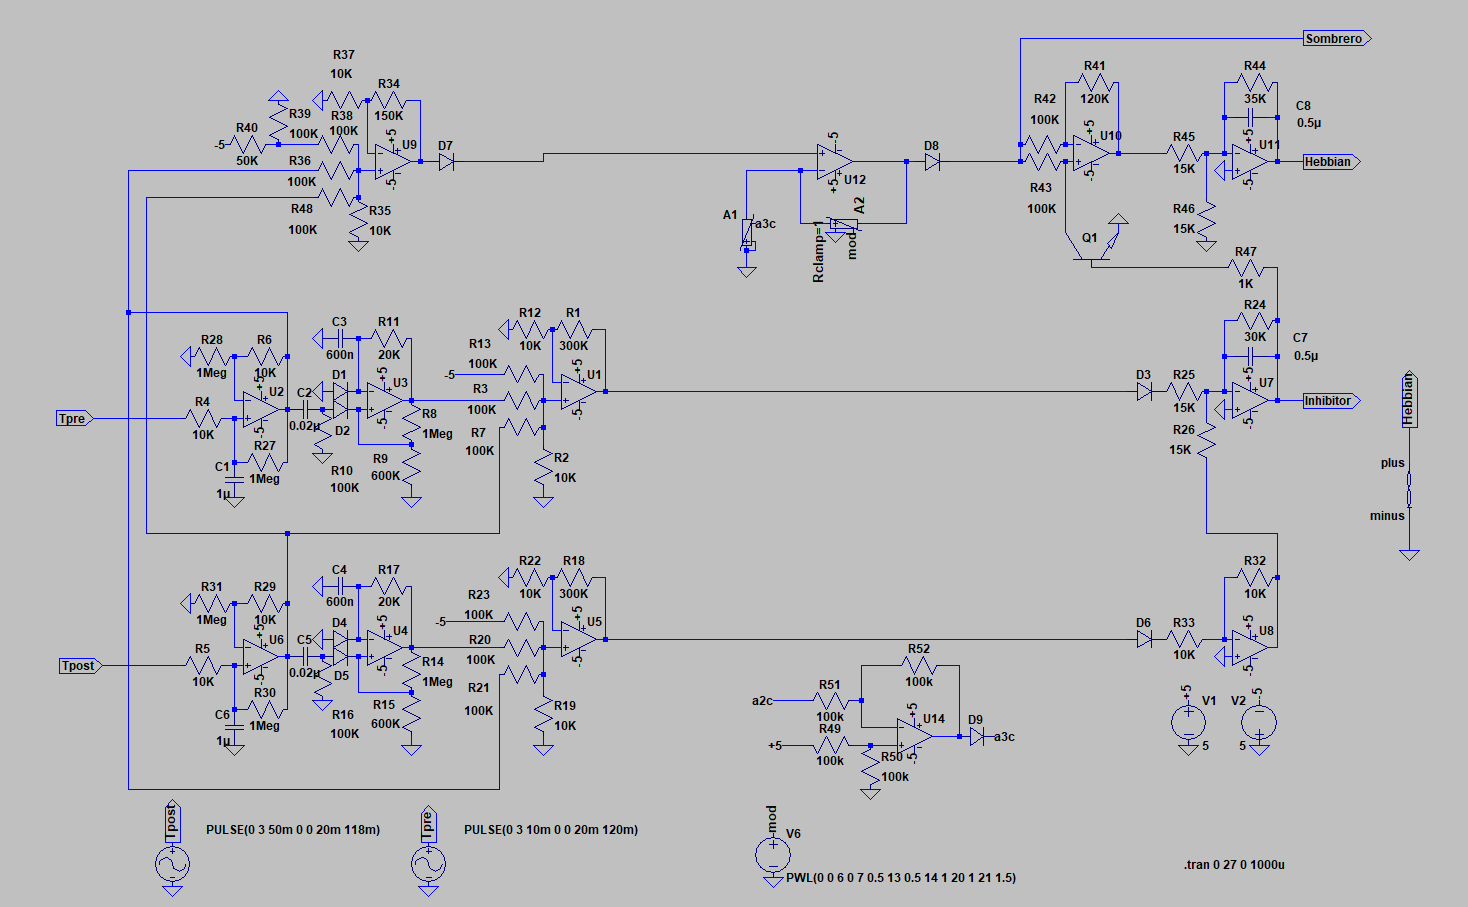
\includegraphics[width=0.8\linewidth]{da_modulation_sch}
\end{figure}
\end{frame}

%------------------------------------------------
\section{DA modulation simulation}
%------------------------------------------------

\begin{frame}
\frametitle{DA modulation: simulation results}
\begin{figure}
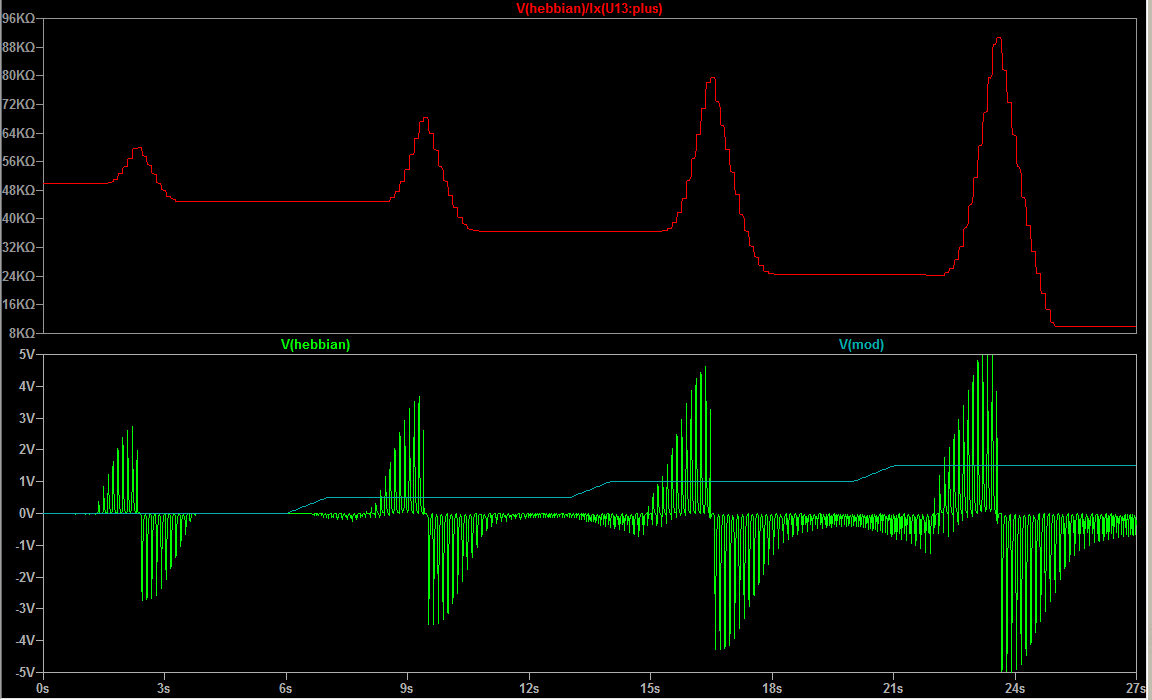
\includegraphics[width=0.8\linewidth]{da_modulation}
\end{figure}
\end{frame}

%------------------------------------------------
\section{Experiments}
%------------------------------------------------

\begin{frame}
  \frametitle{DA modulation: experimental setup}
\begin{figure}
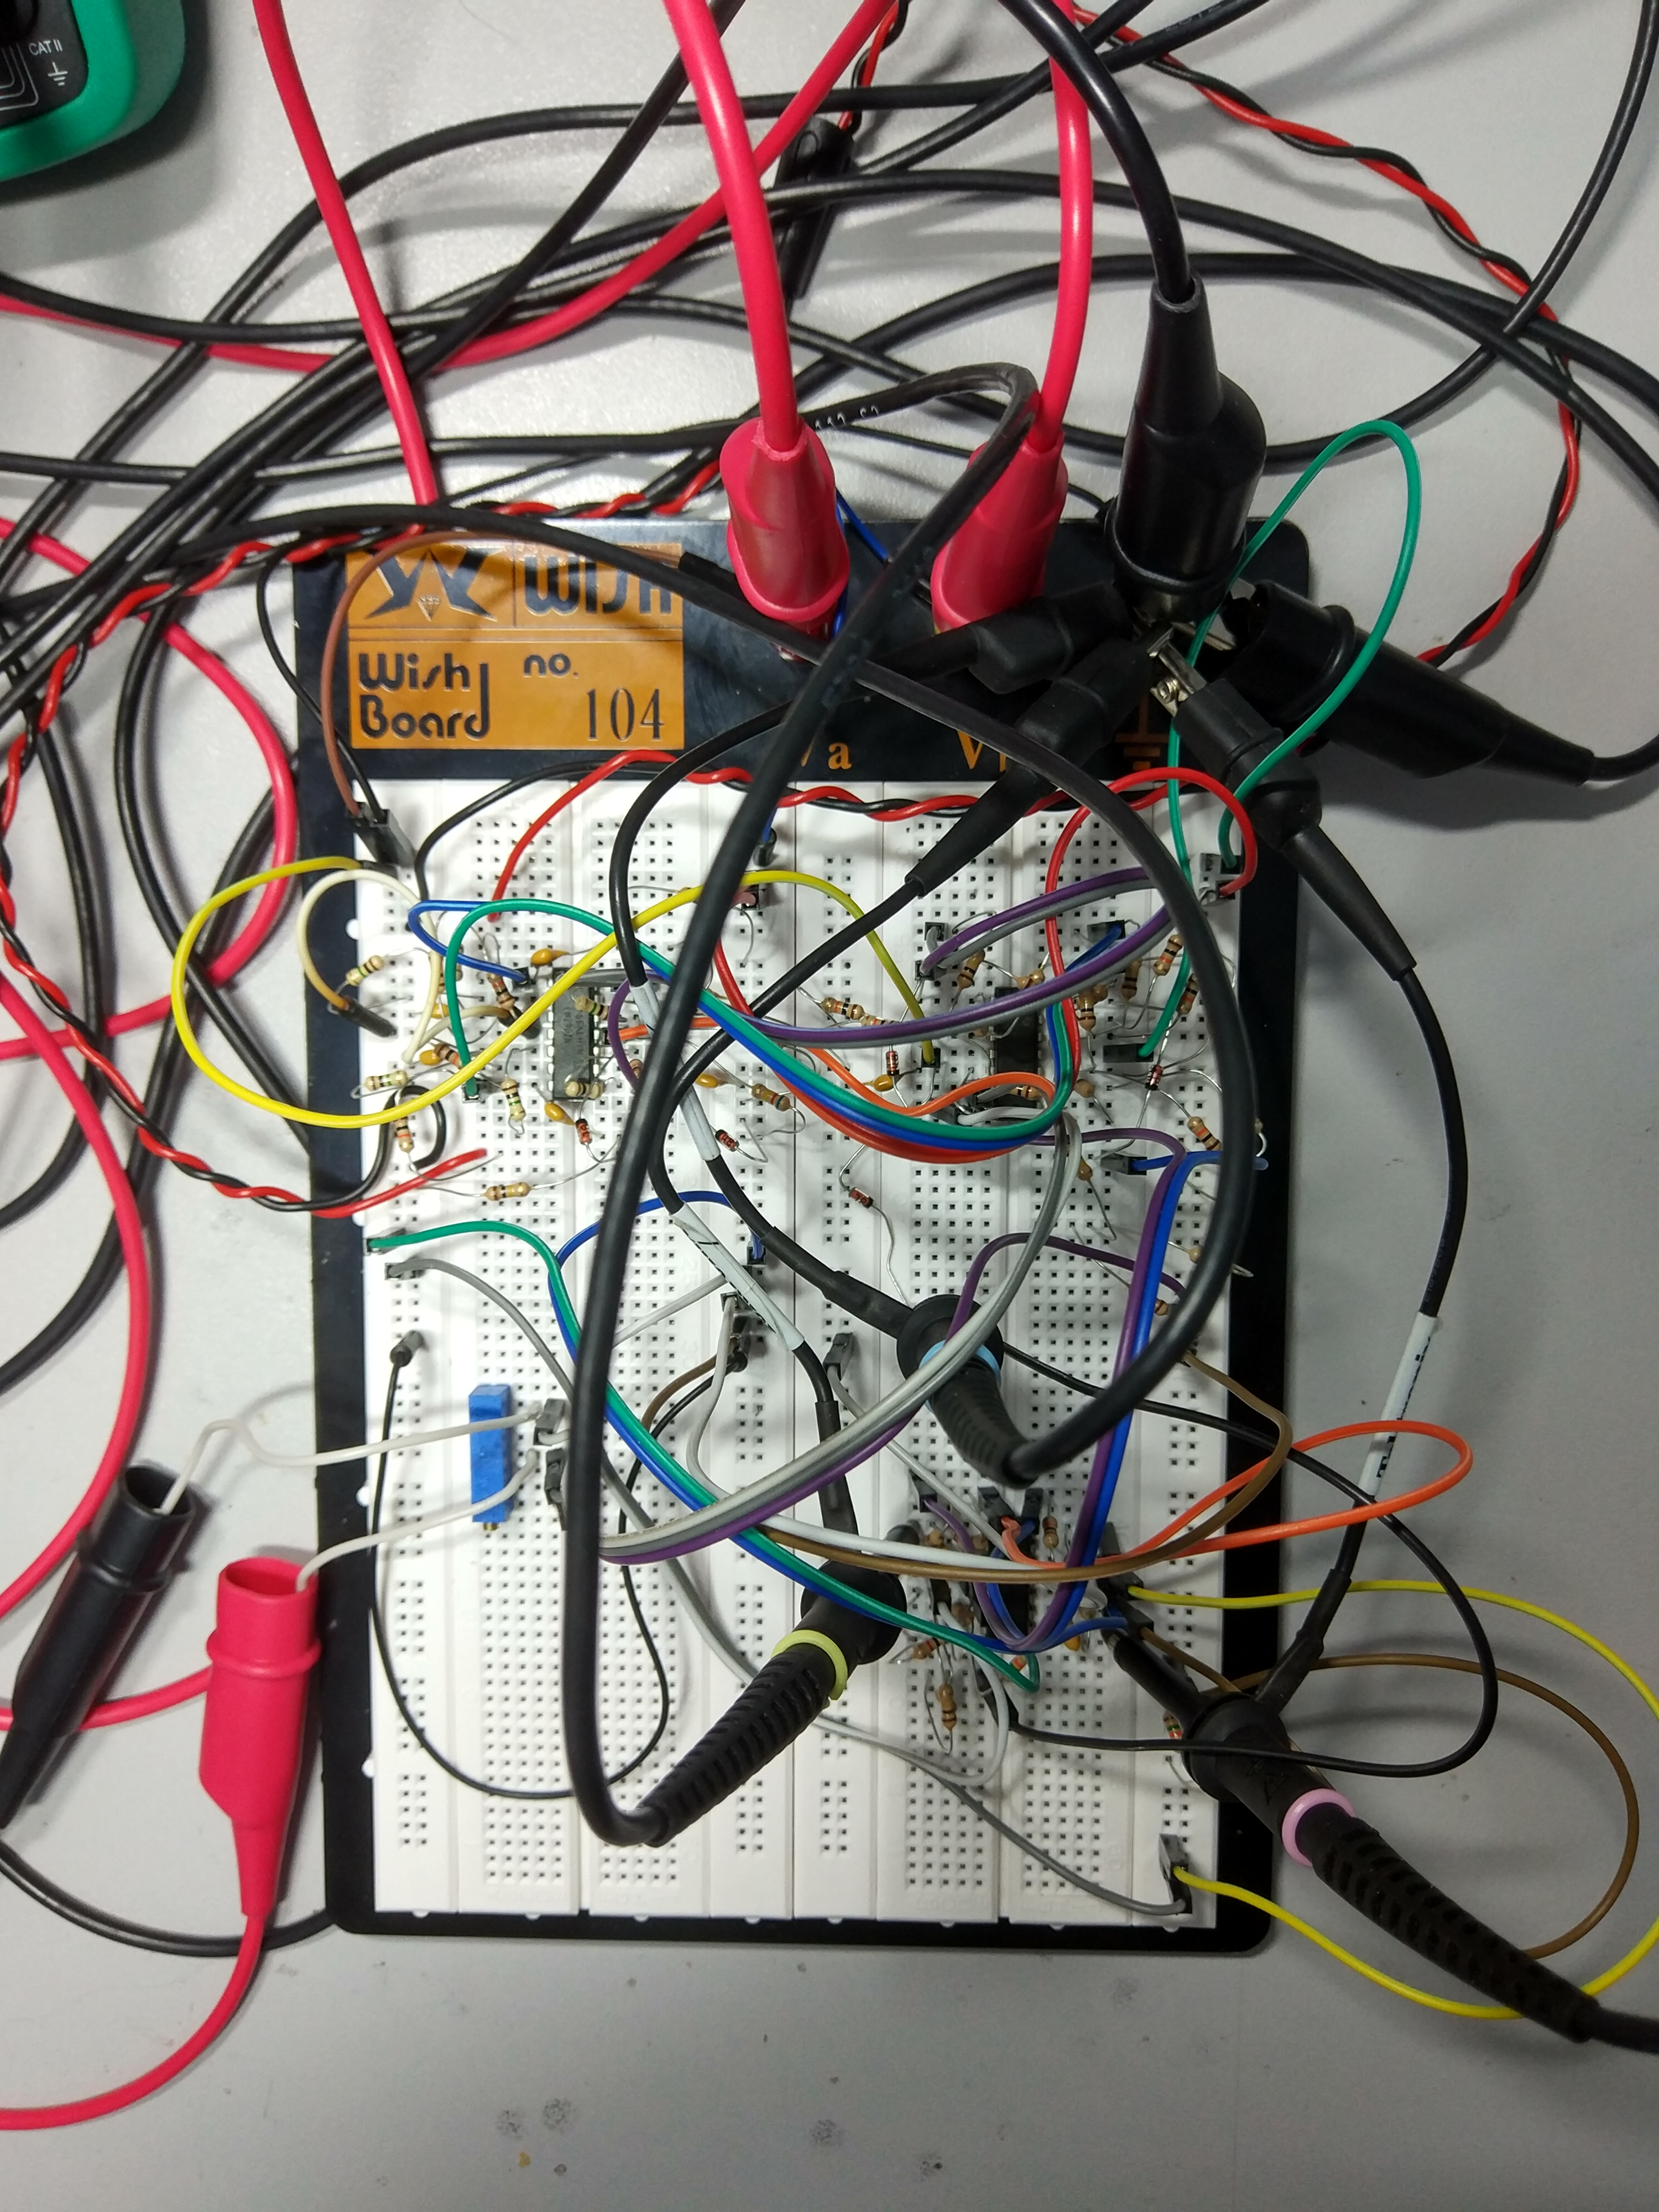
\includegraphics[width=0.5\linewidth, angle=90]{DA_STDP_modulation_physical_schematic}
\end{figure}
\end{frame}

%------------------------------------------------

%------------------------------------------------
\subsection{iSTDP results}
%------------------------------------------------

\begin{frame}
\frametitle{Hebbian STDP; iSTDP}
\begin{columns}[c] % The "c" option specifies centered vertical alignment while the "t" option is used for top vertical alignment

\column{.5\textwidth} % Left column and width
%------------------------------------------------
\begin{figure}
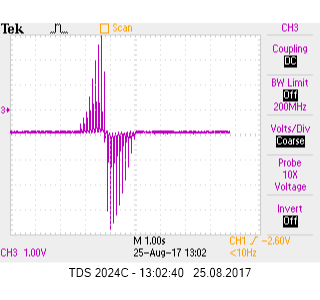
\includegraphics[width=1\linewidth]{hebb_output_single}
\end{figure}
%------------------------------------------------
\column{.5\textwidth} % Right column and width
%------------------------------------------------
\begin{figure}
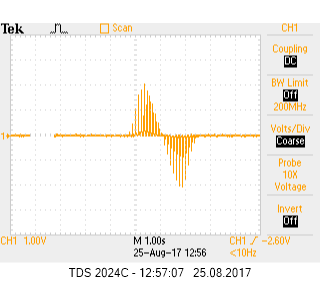
\includegraphics[width=1\linewidth]{inh_output_single}
\end{figure}
%------------------------------------------------
\end{columns}
\end{frame}

%------------------------------------------------
\subsection{DA modulation results}
%------------------------------------------------

\begin{frame}
  \frametitle{DA modulation: results}
  
\begin{figure}
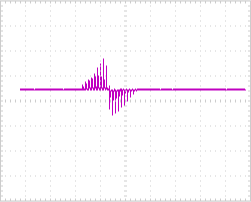
\includegraphics[width=0.33\linewidth]{hebb_r_0_50K}
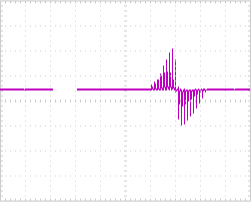
\includegraphics[width=0.33\linewidth]{hebb_r_25_25K}
\end{figure}
\begin{figure}
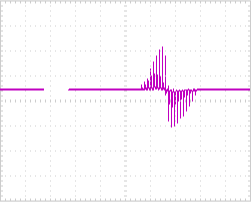
\includegraphics[width=0.33\linewidth]{hebb_r_37_5_12_5K}
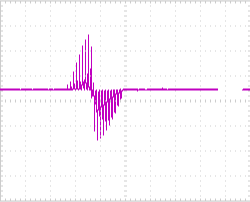
\includegraphics[width=0.33\linewidth]{hebb_r_50_0K}
\end{figure}

\end{frame}

%------------------------------------------------

\begin{frame}
  \frametitle{Memristive brain references}
\begin{columns}[c]
\column{.5\textwidth} % Left column and width

Repository:\\
\url{https://github.com/research-team/memristive-brain}\\


Latest technical report:\\
\url{https://arxiv.org/abs/1709.06325}

\column{.4\textwidth} % Right column and width
\begin{figure}
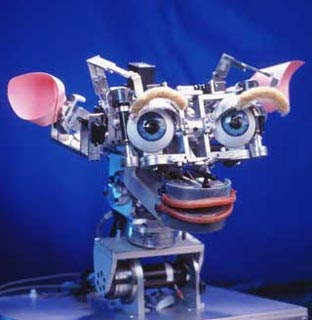
\includegraphics[width=1.0\linewidth]{Kismet_312}
\end{figure}
\end{columns}
\end{frame}

%------------------------------------------------
\section{Supplementary slides}
%------------------------------------------------
\begin{frame}
\frametitle{DA modulation}
\begin{figure}
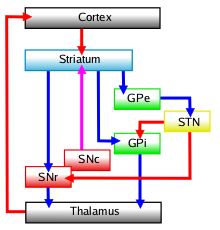
\includegraphics[width=0.5\linewidth]{nigrostriatal}
\end{figure}
\end{frame}
%------------------------------------------------
\begin{frame}
\frametitle{DA implementation}
\begin{figure}
\includegraphics[width=0.7\linewidth]{dopamine_diagram}
\end{figure}
\end{frame}
%------------------------------------------------
\begin{frame}
\frametitle{5-HT implementation}
\begin{figure}
\includegraphics[width=0.7\linewidth]{serotonin_diagram}
\end{figure}
\end{frame}
%------------------------------------------------


\end{document} 
